\documentclass[letterpaper,10pt,onecolumn,titlepage]{article}

\usepackage{graphicx}          
\usepackage{epstopdf}                              
\usepackage{amssymb}                                         
\usepackage{amsmath}                                         
\usepackage{amsthm}                                          

\usepackage{alltt}                                           
\usepackage{float}
\usepackage{color}
\usepackage{url}

\usepackage{balance}
\usepackage[TABBOTCAP, tight]{subfigure}
\usepackage{enumitem}


\usepackage{geometry}
\geometry{textheight=8.5in, textwidth=6in}

%random comment

\newcommand{\cred}[1]{{\color{red}#1}}
\newcommand{\cblue}[1]{{\color{blue}#1}}

\usepackage{hyperref}
\usepackage{geometry}

\def\name{Marty Ulrich}

%% The following metadata will show up in the PDF properties
\hypersetup{
  colorlinks = true,
  urlcolor = black,
  pdfauthor = {\name},
  pdfkeywords = {cs311 ``operating systems'' files pipes processes},
  pdftitle = {CS 311 Assignment 3: Threads},
  pdfsubject = {CS 311 Assignment 3},
  pdfpagemode = UseNone
}

\begin{document}

\title{Assignment 3}
\author{Marty Ulrich\\
Oregon State University - CS 311}
\renewcommand{\today}{March 1, 2012}
\maketitle

\section {Overview}
This program finds all prime numbers between one and a number taken as a command line argument between one and 2\^32.  It prints out the number of primes in the range, and prints the numbers to an output file named $\emph{primes.txt}$.  


\section {Functions}
	The program contains one source file called "main.cpp".  This file contains four functions that each handle a separate task.  They are: main(), bit\_indexes\_from\_number(), print\_bitmap(), check\_if\_bit\_index\_is\_prime().

	\subsection {main()}
	The main() function handles the program.  It should probably have been split into more functions, but none of them seemed large enough to need their own function.  All the thread creating is done here, so the function acts as a sort of home base for the other threads.

	\subsection{bit\_indexes\_from\_number()}
	This function takes in an unsigned long long int and decides what the indexes of the number will be to locate the bit in the bitmap.  The first component of the two values it returns is the index of the long long that the bit is in.  The second component is the offset in that long long.

	\subsection{print\_bitmap()}
	This function prints the contents of the bitmap such that bits set to 0 are written to the output file containing all the primes.  It also prints out the the screen the number of primes in the range.

	\subsection{check\_if\_bit\_index\_is\_prime()}
	This function simply takes in the index returned from bit\_indexes\_from\_number() and checks if the value is set to 0.


\section{Design}
	The program works by iterating through the list if numbers (represented as a bitmap) and when it finds a 0 bit, determines that number is a prime, and creates threads to mark its multiples as 1, representing non-primes.

\section {Work Log}
\begin{center}
    \begin{tabular}{ | l | p{5cm} |}
    \hline


Tue Feb 14 20:26:31 2012 & Working. \\ \hline
Mon Feb 23 21:23:49 2012 & Increasing number of threads decreases total amount of time it takes, but total number of primes is off by a couple. \\ \hline
Mon Feb 23 20:08:20 2012  & Changed the method used to find primes back to the way it originally was, hopefully this time it works better. \\ \hline
Mon Feb 24 17:34:19 2012 & Working most of the time, with parallelization, getting faster with more threads, but not always getting right number of primes. \\ \hline
Mon Feb 24 16:35:26 2012 & WORKING VERSION.  Making optimizations. \\ \hline
Sun Feb 27 22:24:09 2012 & Parellel working with some amounts of threads, but not all. \\ \hline
Sun Feb 27 20:32:22 2012 & Works with one thread.  adding parallel. \\ \hline
Sun Feb 28 20:32:22 2012 & Everything works. \\ \hline
    \end{tabular}
\end{center}

\begin{figure}[b]
	\centering
 	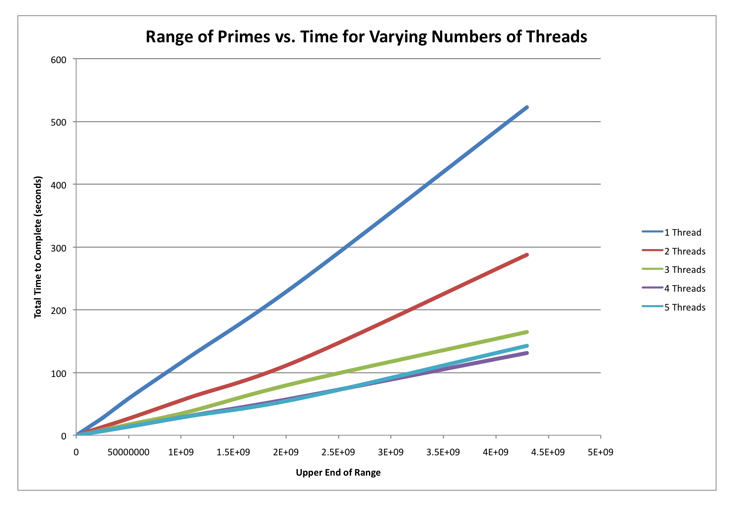
\includegraphics{graph}
	  \caption{A graph of time vs file size}
\end{figure}


\end{document}